% !Mode:: "TeX:UTF-8"
% !TEX program  = xelatex
\documentclass[a4paper]{article}
\usepackage{amsmath}
\usepackage{amssymb}
\usepackage{ctex}
\usepackage{graphicx}
\usepackage{subfigure}
%\usepackage{braket}
\usepackage[european]{circuitikz}
\usepackage{multirow}
\usepackage{geometry}
\usepackage{float}
\geometry{left=2.5cm,right=2.5cm,bottom=2.5cm,top=2.5cm}
\title{物理化学实验: 分子偶极矩的测试}
\author{薛明怡\quad 151250177\quad 化学化工学院}
\date{\today}
\begin{document}
\maketitle
%%\tableofcontents
%%\bibliographystyle{unsrt}
\section{实验目的}
\begin{enumerate}
\item 用电桥法测定极性物质(乙酸乙酯)在非极性溶剂(环己烷)中的介电常数和分子偶极矩.
\item 了解分子偶极矩与分子电性质的关系, 溶液法测定偶极矩的实验原理.
\end{enumerate}
\section{实验原理}
\subsection{偶极矩}
分子是独立存在, 相对稳定, 能保持物理化学特性的最小单元. 
分子由带正电的原子实和带负电的价电子云构成. 
由于化学键的极性以及分子结构的不对称性, 正电几何中心和负电几何中心常常不重合,
产生了分子的偶极矩, 具有偶极矩的分子也被称为极性分子. 偶极矩的定义如下,
\begin{equation}
	\mu = q \cdot d
\end{equation}
\begin{figure}[H]
	\begin{center}
		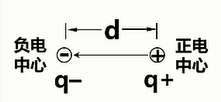
\includegraphics[width = 0.3\paperwidth]{fig/definition.png}
	\end{center}
	\caption{偶极矩的定义}
\end{figure}
分子偶极矩的作用: 
\begin{enumerate}
	\item 极性分子在低频电场的作用下会产生一定的取向(极化现象), 应用: 液晶分子在电场作用下极化
	\item 极性分子靠近时偶极电场产生额外的分子间相互作用, 应用: 设计晶体
	\item 取向排列的分子可以产生额外的附加电场, 应用: 非线性光学, 压电效应
	\item 偶极矩测试可以用于判断共价键极性, 分子极性, 分子结构对称性
\end{enumerate}
\begin{figure}[H]
	\centering
	
\includegraphics[width = 0.5\paperwidth]{fig/logic.png}
	\caption{实验的逻辑}
\end{figure}
\subsection{摩尔极化度}
如存在外加电场$E$, 则极性分子的骨架, 电子云与转动取向会随电场做出相应的调整, 
这种调整使体系能量降低, 有序性增加, 称为极化现象.
\par
总的极化度$P$由上述三种效应线性叠加在一起, 其中分子骨架和电子云的极化被称为
变形极化$P_{tf}$, 偶极转动取向产生的极化被称为转向极化$P_{rot}$. 电子云, 分子骨架, 转向取向
三种极化过程需要的时间逐渐增加, 因此通过比较$> 10^{15}$Hz的紫外可见高频电场, 
$10^{12}-10^{14}$Hz红外中频电场以及$< 10^{10}$Hz低频电场作用下物质总极化度
的差异, 可以区分三种极化度的各自贡献.
\begin{equation}
	P = P_{tf}+P_{rot}
\end{equation}
\begin{figure}[H]
	\begin{minipage}[t]{0.5\linewidth}
		\centering
		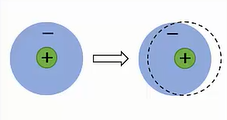
\includegraphics[width=2.2in]{fig/electron_disform.png}
		\caption{电子云变形}
		\label{fig:side:a}
	\end{minipage}
	\begin{minipage}[t]{0.5\linewidth}
		\centering
		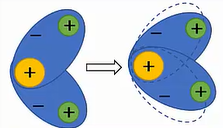
\includegraphics[width=2.2in]{fig/frame_disform.png}
		\caption{骨架变形}
		\label{fig:side:b}
	\end{minipage}
\end{figure}
转动取向需要的时间最长, 当外加电场频率超过红外中频后, 
分子转动速度跟不上电场的切换速度, 因此只有在低频电场或分子处于气相液相等
自由状态下.
\par
电场使极化分子发生转向极化, 极化后能量降低正比于
$\vec{E}\cdot \vec{\mu}$, 分子的随即热运动($k_{b}T$)会破坏
转向极化. 两者之间的平衡关系符合统计力学玻尔兹曼分布. 
以此为基础导出摩尔转向极化度和分子偶极矩之间的关系, 
\begin{equation}
	P_{rot} = \frac{N}{3\epsilon_{0}}\cdot \frac{\mu^{2}}{3k_{b}T}
\end{equation}
\subsection{介电常数}
极化现象是电解质的基本性质, 构成电介质的分子极化度决定了材料的介电常数
$\epsilon$. Clausius, Mosott和Debye基于经典电动力学推导出理想气体中介电常数
与分子极化度的关系, 也就是克劳修斯-莫索提-德拜方程,
\begin{equation}
	P = \frac{\epsilon_{r}-1}{\epsilon_{r}+2}\cdot \frac{M}{\rho}
\end{equation}
式中, $\epsilon_{r}$是相对介电常数, $M$是摩尔质量, $\rho$是密度. 这个公式
建立起分子微观的可极化性$P$与宏观物化性质介电常数$\epsilon$之间的关系.
\par
\subsection{交变电场测定分子偶极矩}
在不同的电场频率下, 分子的可极化性改变, 物质的介电常数也会相应发生变化.
介电性随频率的变化情况也被称为介电谱, 为研究物质内部有关极化机制和晶格振动
等提供重要信息.
\par
对于有机分子体系, 在低频(准静态)电场下的介电常数($\epsilon_{r, low}$)包括
分子变形极化和转向极化的贡献; 高频(可见光)电场下, 分子转向极化无法再跟随
电场的变化, 因此介电常数$\epsilon_{r, high}$仅包括分子变形极化的贡献. 
理论上, 通过$\epsilon_{r, high} - \epsilon_{r, low}$可以推算出分子转向极化度
($P_{rot}$), 从而通过公式3确定分子偶极矩$\mu$.
\par
低频下物质的相对介电常数可通过电容法测定, 
\begin{equation}
	\epsilon_{r, low} = \frac{C}{C_{0}}
\end{equation}
在相对磁导率约为1的前提下, 高频介电常数与折射率$n$有如下关系,
\begin{equation}
	\epsilon_{r, high} = n^{2}
\end{equation}
折射率$n$可通过阿贝折光仪测定.
\subsection{极稀溶液近似}
对于公式3和公式4, 推导过程中忽略了分子间的相互作用力, 
也就是说公式仅适用于理想气体状态. 在实际应用中, 处于气态的
极性分子毕竟是少数. 在液态极性分子之间的偶极矩相互租用会使
$\epsilon-P-\mu$三者关系更加复杂, 方程不再成立.
\par
由于偶极-偶极分子相互作用随分子距离的二次方衰减, 因此人们使用
非极性分子作为分散溶剂, 采用极稀溶液极限近似忽略极性分子间
的相互作用力, 模拟气体状态.
\par
稀溶液的各项物化性质随溶质浓度变化可用简单的线性公式来描述, 
\begin{equation}
	\centering
	\begin{aligned}
		\epsilon_{r, sol} &= \epsilon_{r1}(1+\alpha x_{2})\\
		\rho_{sol} &= \rho_{1}(1+\beta x_{2})\\
		n_{sol} &= n_{1}(1+\gamma x_{2})\\
	\end{aligned}
\end{equation}
其中, $\epsilon_{r, sol}$为溶液的相对介电常数, $\epsilon_{r1}$为溶剂
的相对介电常数, $x_{2}$为溶质的摩尔分数, $\rho_{sol}$为溶液的密度, 
$\rho_{1}$为溶剂的密度, $n_{sol}$为溶液的折射率, $n_{1}$为溶剂的折射率, 
$\alpha$, $\beta$, $\gamma$均为实测参数.
\par
溶液的摩尔极化度具有加和性, 与溶剂和溶质的摩尔极化度的摩尔分数有关
$P_{sol} = x_{1}P_{1}+x_{2}P_{2}$, 
结合公式4, 5, 6, 7, 并求溶质摩尔分数$x_{2}$趋于0时$P$值的数学极限, 
\begin{equation}
	\centering
	\begin{aligned}
		P &= P_{2}^{\infty} = \lim\limits_{x_{2}\to 0} P_{2}\\
	  &=\frac{3\alpha\epsilon_{r1}}{(\epsilon_{r1}+2)^{2}}\cdot \frac{M_{1}}{\rho_{1}}
	  + \frac{\epsilon_{r1}-1}{\epsilon_{r1}+2}\cdot \frac{M_{2}-\beta M_{1}}{\rho_{1}}\\
	P_{elec} &= R_{2}^{\infty} = \lim\limits_{x_{2}\to 0}R_{2}\\
			 &=\frac{n_{1}^{2}-1}{n_{1}^{2}+2}\cdot \frac{M_{2}-\beta M_{1}}{\rho_{1}}
			 +\frac{6n_{1}^{2}M_{1}\gamma}{(n_{1}^{2}+2)^{2}\rho_{1}}\\
	\end{aligned}
\end{equation}
\par
结合稀溶液极限下摩尔极化度$P_{2}^{\infty}$, 电子云变形摩尔极化度
$R_{2}^{\infty}$的计算公式, 作差得到转向极化度$P_{rot}$, 转向极化度
通过公式3与偶极矩建立联系, 带入参数得到以下公式, 
\begin{equation}
	\centering
	\begin{aligned}
		P_{rot} &= P_{2}^{\infty} - R_{2}^{\infty}\\
				&=\frac{N}{3\epsilon_{0}}\cdot \frac{\mu^{2}}{3k_{b}T}\\
		\mu &= 0.0426\times 10^{-30} \sqrt{(P_{2}^{\infty} - R_{2}^{\infty})T}\\
	\end{aligned}
\end{equation}
\par
需要实验测定的参量有$\alpha$, $\beta$, $\gamma$, 溶剂折射率, 溶剂密度以及溶剂介电常数.
\section{仪器与药品}
\begin{enumerate}
	\item \textbf{仪器:} 阿贝折射仪, 精密电容测量仪, 台灯, 擦镜纸, 
	10mL小烧杯5只, 25mL烧杯, 5mL刻度移液管, 5mL注射器, 25mL容量瓶5只, 5支滴管, 密度管, 洗耳球
    \item \textbf{药品:} 乙酸乙酯, 环己烷, 丙酮, 水
\end{enumerate}
\section{实验步骤}
\subsection{溶液的配制}
通过称重法配置摩尔分数分别为$0.05$, $0.10$, $0.15$, $0.20$, $0.30$的乙酸乙酯/环己烷溶液.
\begin{enumerate}
	\item 将容量瓶吹干, 放入天平, 待示数稳定后, 记下容量瓶的质量, 去皮.
	\item 按所需量移取乙酸乙酯(可通过移液管移取相应体积再称重), 记录乙酸乙酯质量.
	\item 加入环己烷定容至刻度线, 均匀混合后称重, 记录乙酸乙酯+环己烷总质量.
\end{enumerate}
\subsection{折射率的测定}
\begin{enumerate}
	\item 测量水的折射率, 重复测试3次, 记录温度和折射率.
	\item 测量待测溶液折射率, 每个样品测量3组数据, 测量有机物后棱镜不需要用丙酮擦拭.
\end{enumerate}
\subsection{相对介电常数的测定}
\begin{enumerate}
	\item 打开精密电容仪开关, 预热10min.
	\item 校零, 将电容池两极分别接入测量仪对应电极接头处.
	\item 用洗耳球吹干电容池电极和底座上的样品室, 将电容池放入底座样品室中,
	待记录稳定后的示数, 重新吹扫电容池电极和底座样品室, 再次测量电容值, 若示数
	不变, 将此数值记录为空气的实测电容值.
	\item 取下电容池, 用移液管移取3mL环己烷加入样品室中, 放入电容池电极, 待数值
	稳定后, 记录该样品的电容值; 取下电容池, 用针筒将样品室中的液体抽出, 
	放入废液瓶中.
	\item 用洗耳球吹干样品室和洗耳球电极, 测量电容值直到恢复空气实测电容值.
	\item 按上述步骤测量各浓度乙酸乙酯-环己烷溶液的电容值.
\end{enumerate}
\subsection{密度的测定}
\begin{enumerate}
	\item 将密度管洗净, 用丙酮润洗, 在循环水泵上抽干, 可用电吹风加热外壁加快干燥.
	\item 在天平上放入50mL小烧杯, 去皮. 在密度管两端套上磨口帽, 放入烧杯称重.
	记录数值.
	\item 取下磨口帽, 用干净针筒抽取一定去离子水, 从鼓泡一端支管注入密度管中, 
	直至充满整支密度管, 不能有气泡. 鼓泡一端支管稍抬高, 用吸水纸从另一端支管口
	吸去多余的水, 直至鼓泡一端支管液面正好调至刻度线.
	\item 擦干密度管外壁, 套上磨口帽, 称重.
	\item 倒出少量水, 然后补加并调至刻度线, 重复测量1-2次.
	\item 同样方法测量各液体密度, 每次测量前都需先将密度管干燥.
\end{enumerate}
% \newpage
% \section{拓展实验}
\newpage
\section{数据处理}
\subsection{计算$\gamma$}
\begin{figure}[H]
	\centering
	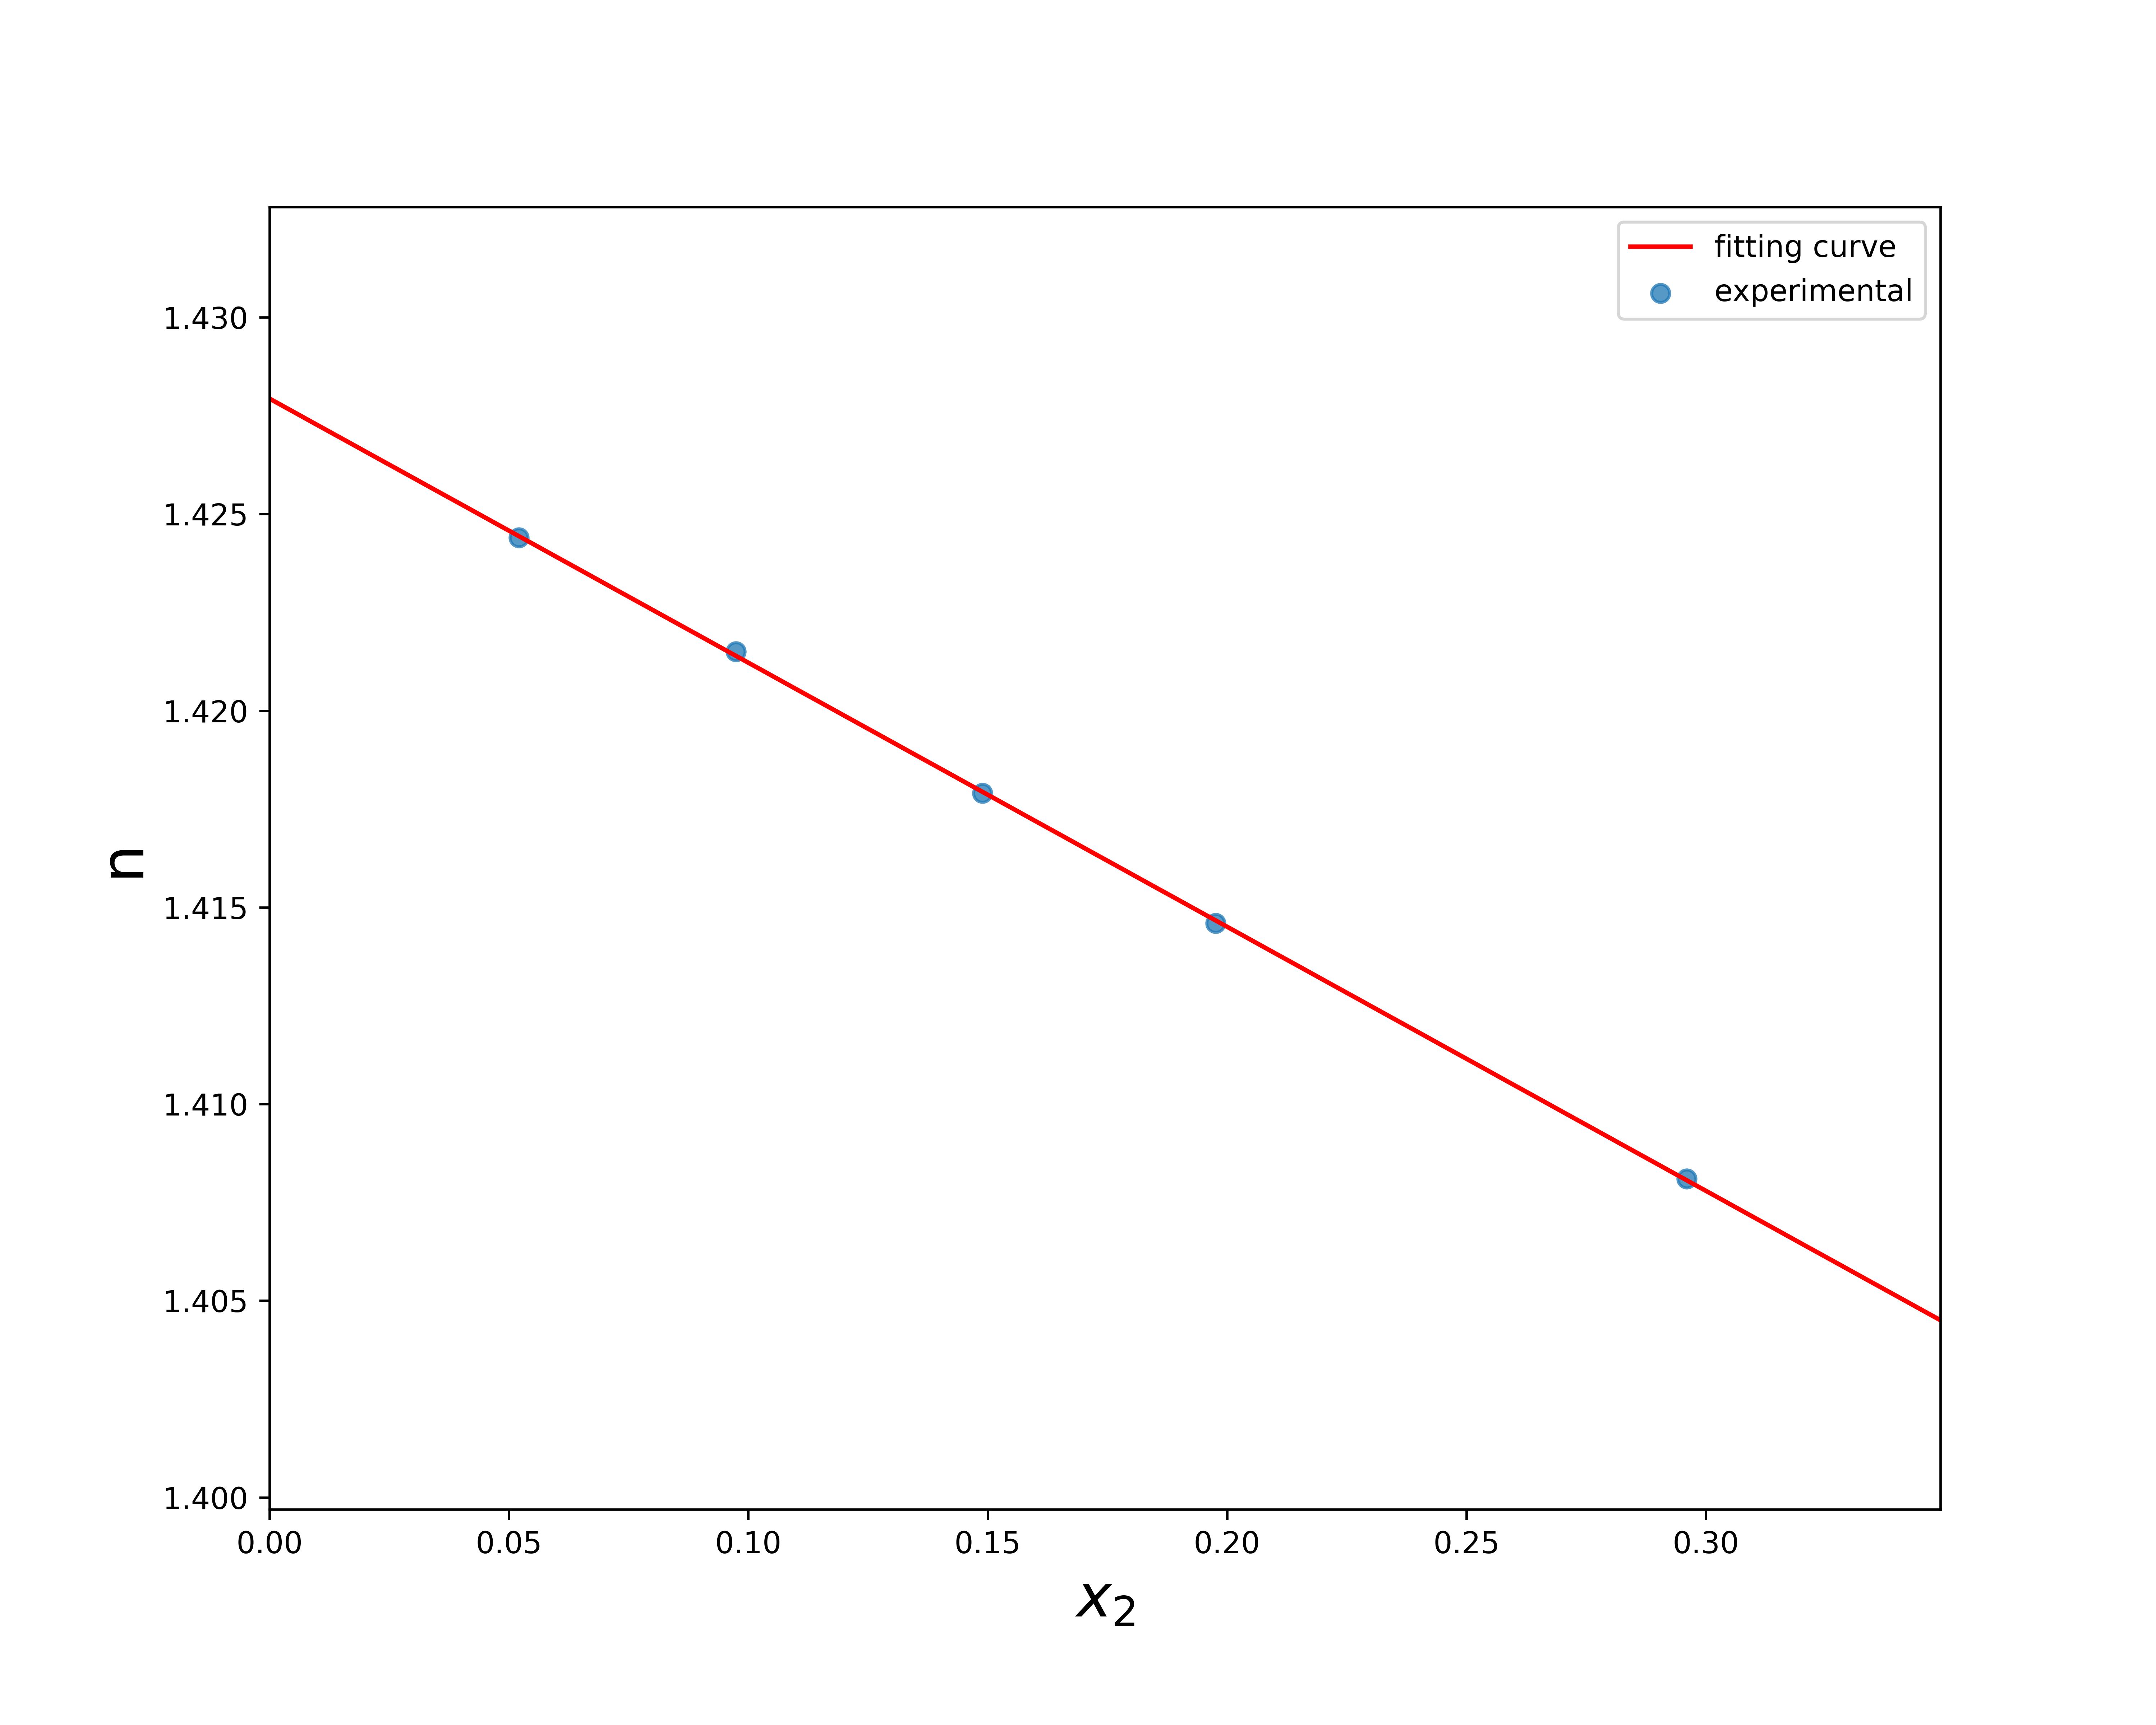
\includegraphics[width = 0.5\paperwidth]{fig/molfraction.png}
	\caption{折光率与摩尔分数曲线}
\end{figure}
\begin{equation}
	\centering
	\begin{aligned}
		n_{sol} &= n_{1}(1+\gamma x_{2})\\
						&= n_{1} + n_{1}\times \gamma x_{2}\\
		n_{1} &= 1.4279\\
		\gamma &= \frac{n_{1}\times \gamma}{n_{1}} = \frac{-0.06712}{1.4279}\\
					&= -0.04701\\
		R^{2} &= 0.9999\\
	\end{aligned}
\end{equation}
\subsection{计算$\beta$}
\begin{figure}[H]
	\centering
	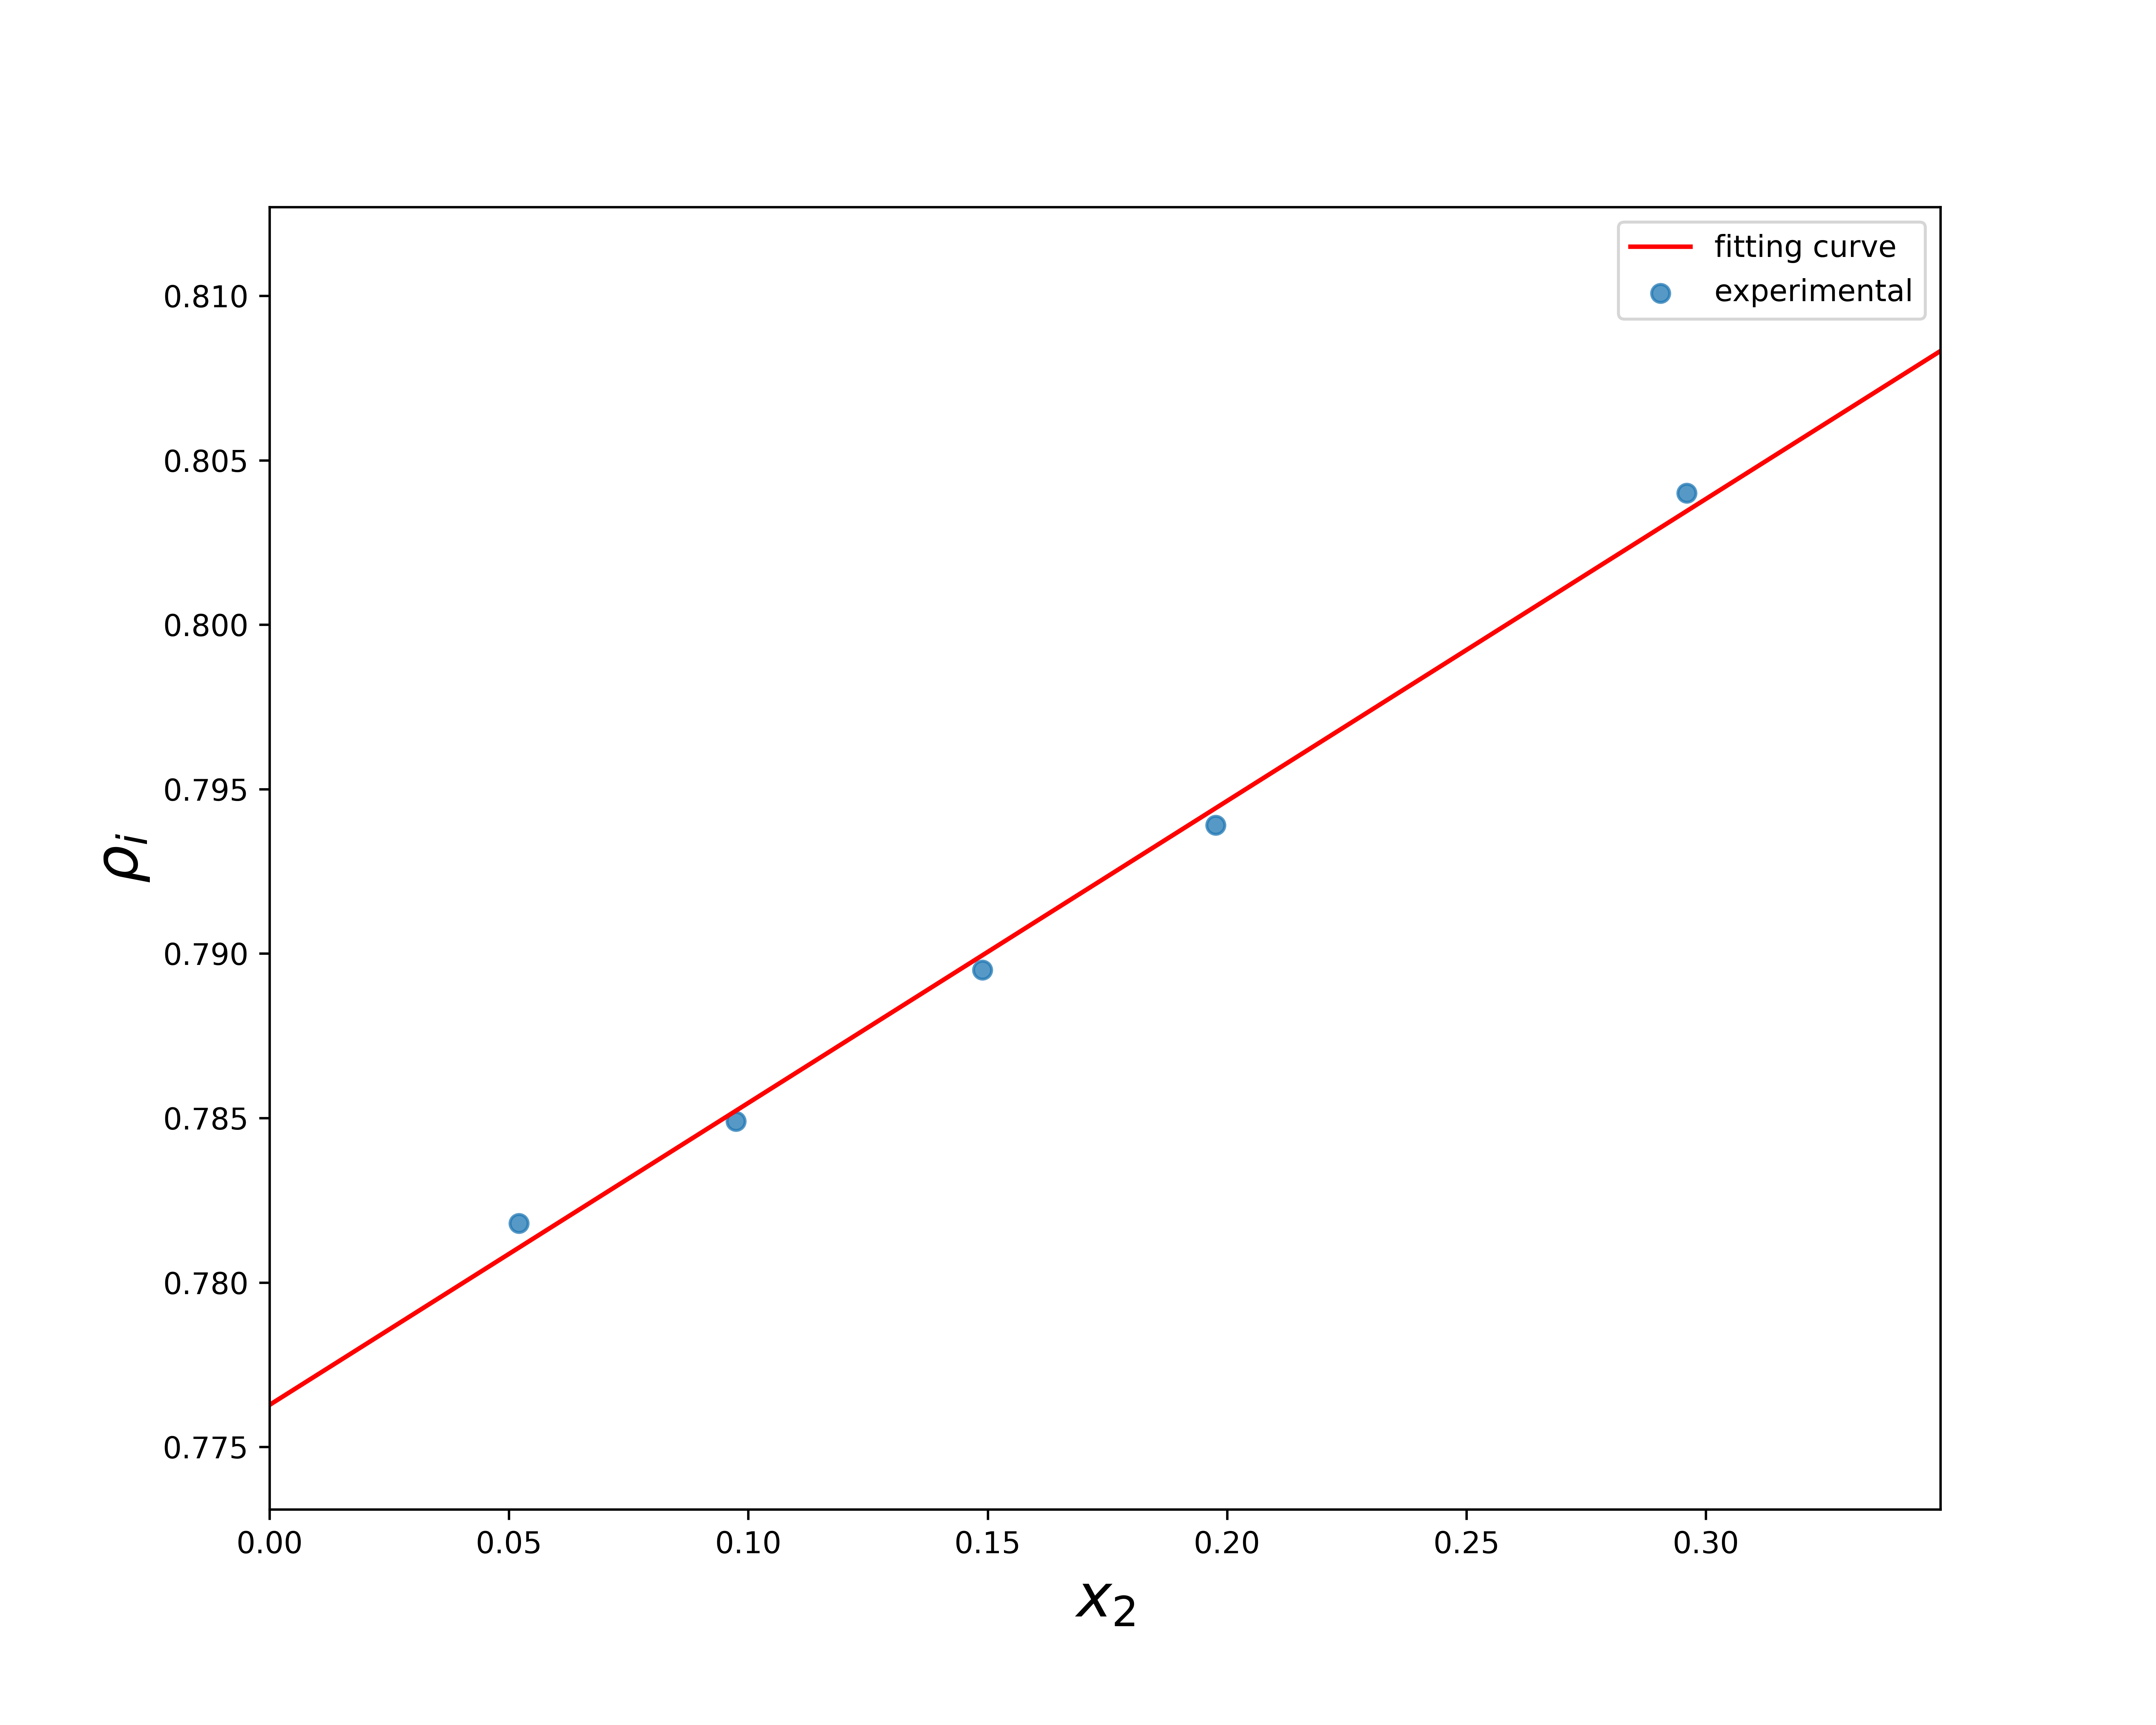
\includegraphics[width = 0.5\paperwidth]{fig/density.png}
	\caption{密度与摩尔分数曲线}
\end{figure}
\begin{equation}
	\centering
	\begin{aligned}
		\rho_{sol} &= \rho_{1}(1+\beta x_{2})\\
							&=\rho_{1} + \rho_{1}\times \beta x_{2}\\
		\rho_{1} &= 0.7763g\cdot cm^{3}\\
		\beta &= \frac{\rho_{1}\times \beta}{\rho_{1}} = \frac{0.09181}{0.7763}\\
					&= 0.1183\\
		R^{2} &= 0.9953\\
	\end{aligned}
\end{equation}
\subsection{计算$\alpha$}
\begin{figure}[H]
	\centering
	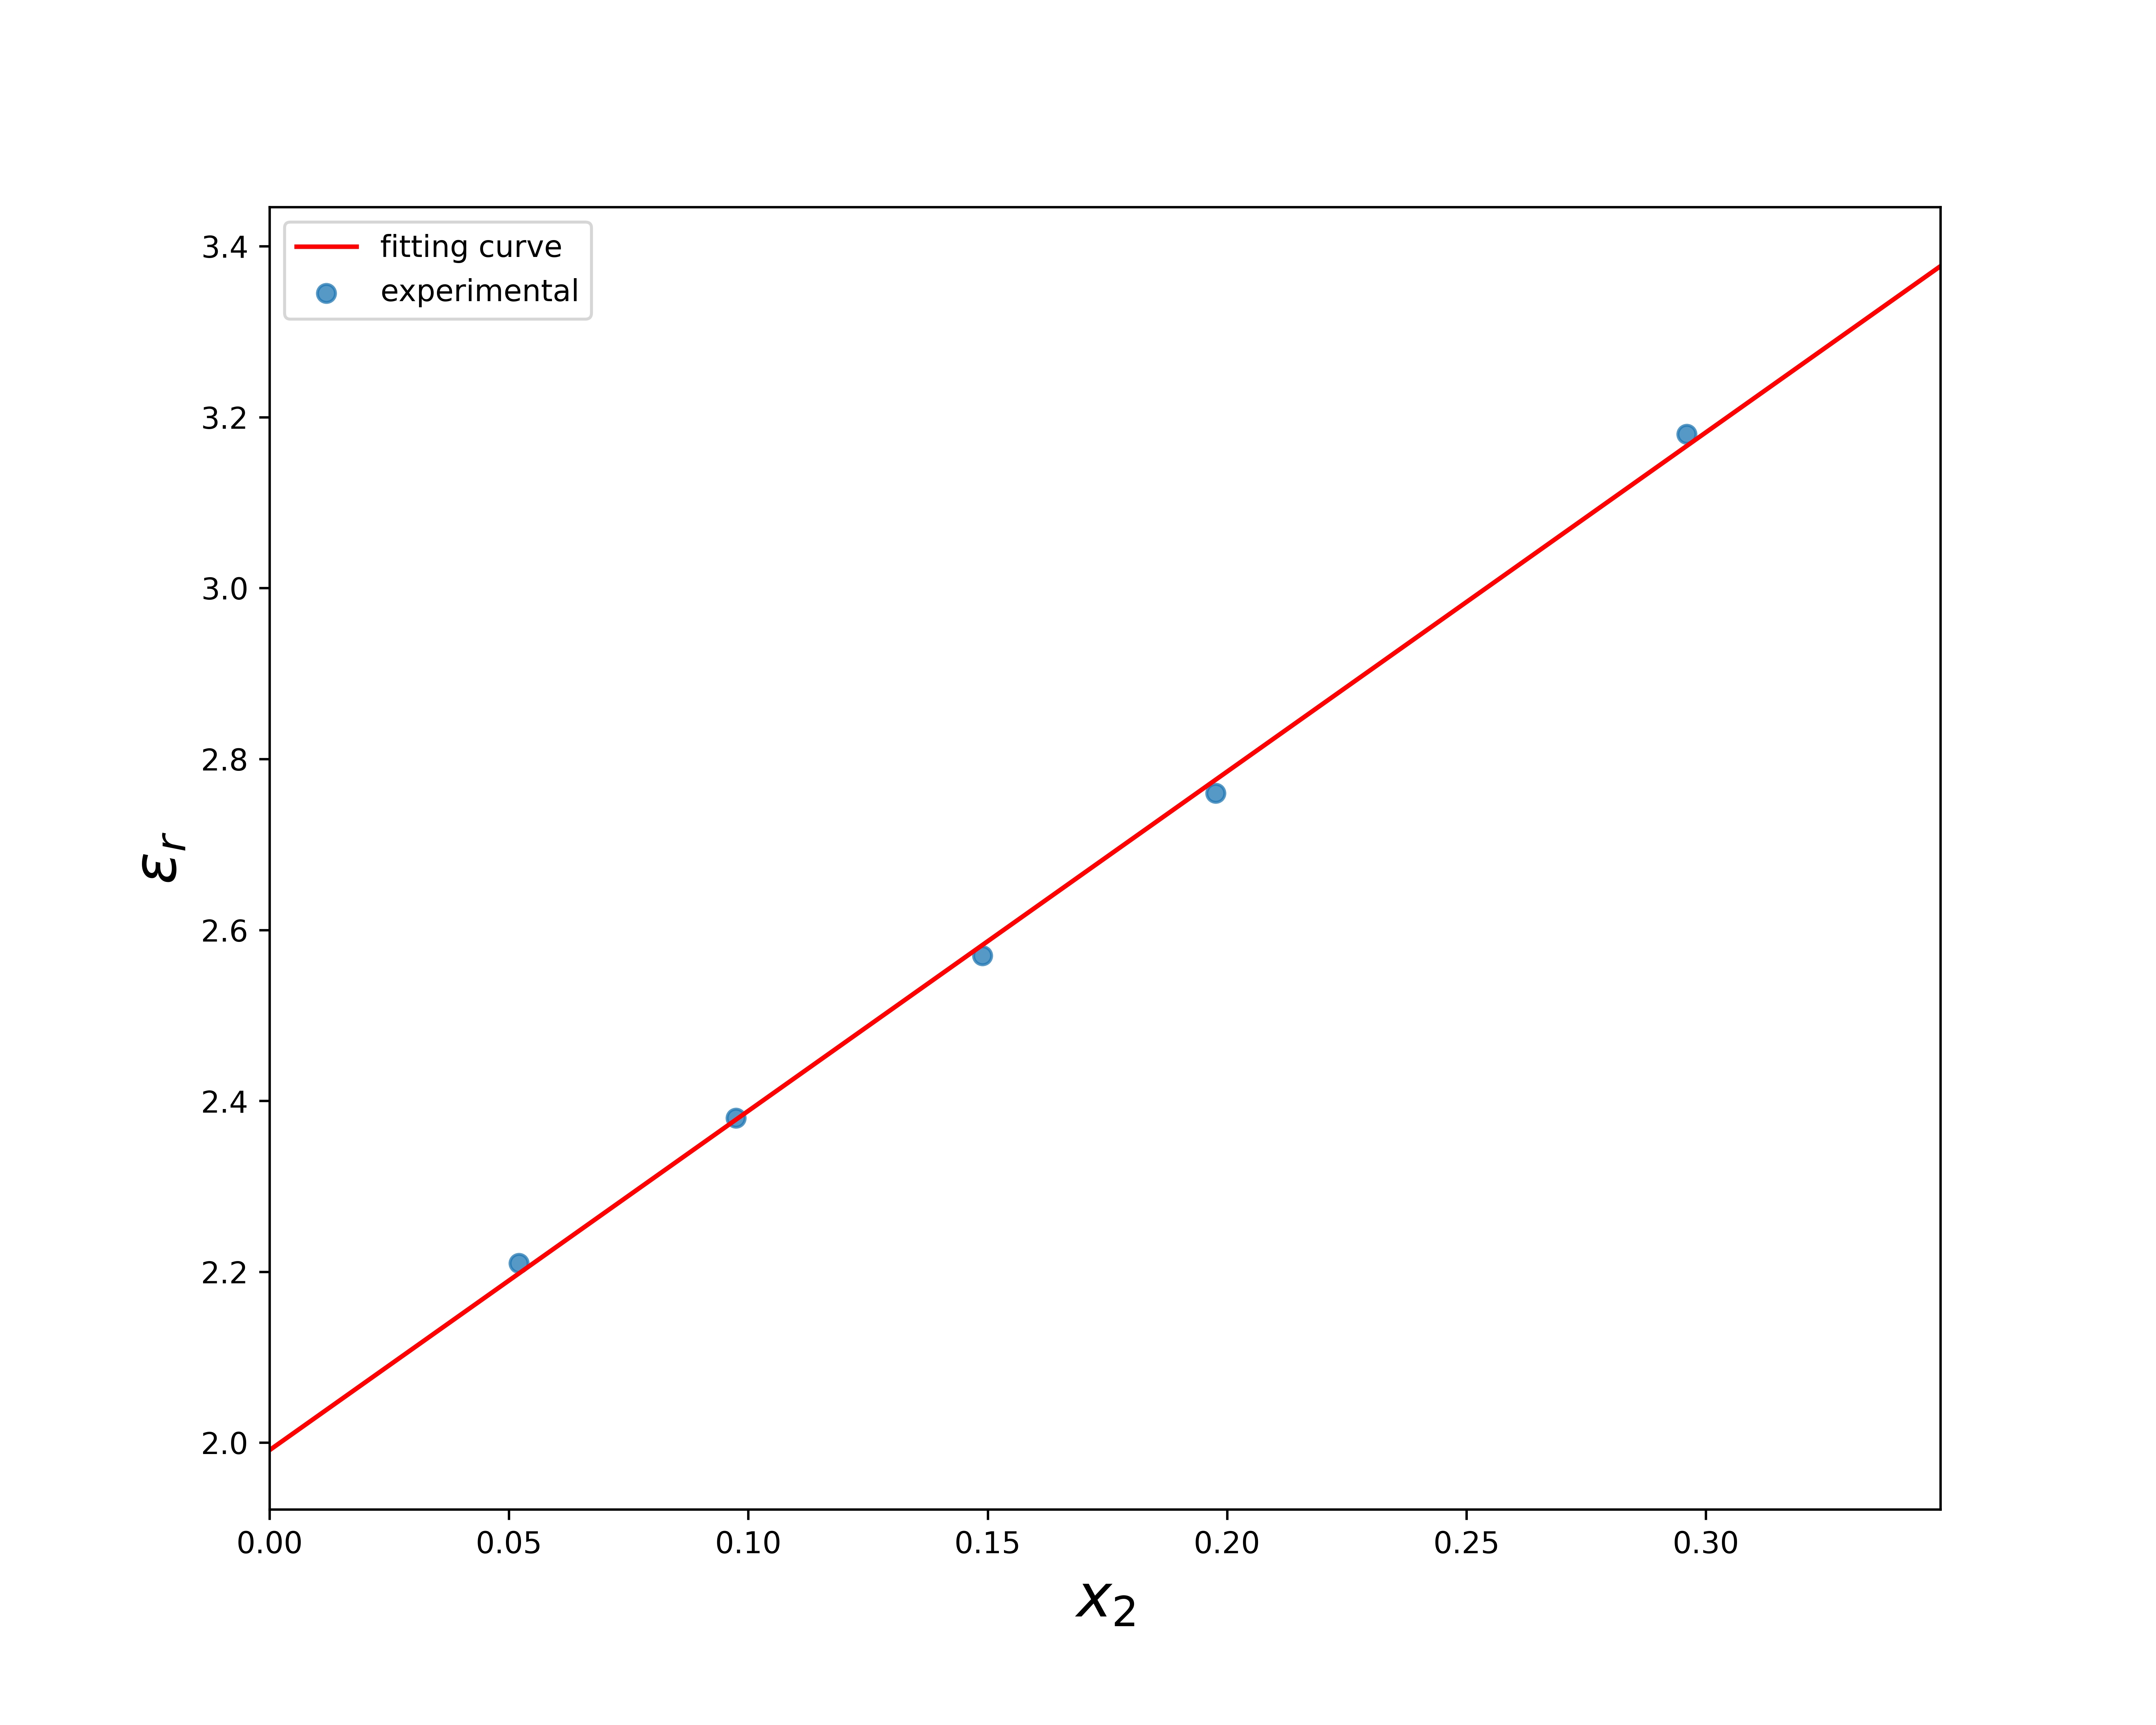
\includegraphics[width = 0.5\paperwidth]{fig/jiedian.png}
	\caption{相对介电常数与摩尔分数曲线}
\end{figure}
\begin{equation}
	\centering
	\begin{aligned}
		\epsilon_{r, sol} &= \epsilon_{r1}(1+\alpha x_{2})\\
											&= \epsilon_{r1}+\epsilon_{r1}\times \alpha x_{2}\\
		\epsilon_{r1} &= 1.9912\\
		\alpha &= \frac{\epsilon_{r1}\times \alpha}{\epsilon_{r1}} = \frac{3.9695}{1.9912}\\
						&= 1.9935\\
		R^{2} &= 0.9987\\
	\end{aligned}
\end{equation}
\subsection{偶极矩的计算}
\begin{equation}
	\centering
	\begin{aligned}
		P &= P_{2}^{\infty} = \lim\limits_{x_{2}\to 0} P_{2}\\
	  &=\frac{3\alpha\epsilon_{r1}}{(\epsilon_{r1}+2)^{2}}\cdot \frac{M_{1}}{\rho_{1}}
		+ \frac{\epsilon_{r1}-1}{\epsilon_{r1}+2}\cdot \frac{M_{2}-\beta M_{1}}{\rho_{1}}\\
		&=\frac{3\times 1.9935\times 1.9912}{(1.9912+2)^{2}}\cdot \frac{84g\cdot mol^{-1}}{0.799g \cdot cm^{-3}}
		+ \frac{1.9912-1}{1.9912+2}\cdot \frac{88g\cdot mol^{-1}-0.1183\times 84g\cdot mol^{-1}}{0.799g \cdot cm^{-3}}\\
		&=102.86cm^{3}\cdot mol^{-1}\\
	P_{elec} &= R_{2}^{\infty} = \lim\limits_{x_{2}\to 0}R_{2}\\
			 &=\frac{n_{1}^{2}-1}{n_{1}^{2}+2}\cdot \frac{M_{2}-\beta M_{1}}{\rho_{1}}
			 +\frac{6n_{1}^{2}M_{1}\gamma}{(n_{1}^{2}+2)^{2}\rho_{1}}\\
			 &=\frac{1.4279^{2}-1}{1.4279^{2}+2}\cdot \frac{88g\cdot mol^{-1}-0.1183\times 84g\cdot mol^{-1}}{0.799g \cdot cm^{-3}}
			 +\frac{6\times 1.4279^{2}\times 84g\cdot mol^{-1}\times (-0.04701)}{(1.4279^{2}+2)^{2}\times 0.799\cdot cm^{-3}}\\
			 &=21.42cm^{3}\cdot mol^{-1}\\
			 \mu &= 0.0426\times 10^{-30} \sqrt{(P_{2}^{\infty} - R_{2}^{\infty})T}\\
			 &=0.0426\times 10^{-30} \sqrt{(102.86-21.42)\times 10^{6}\times (273.15+17.66)} C\cdot m\\
			 &=6.56\times 10^{-27} C\cdot m\\
	\end{aligned}
\end{equation}

					
\newpage
\section{思考与讨论}
\begin{enumerate}
	\item 准确测定溶质的摩尔极化度和摩尔折射度时, 为何要外推至无限稀释?\\
	公式中假定分子间没有相互作用, 因此需要将数据外推至无限稀释后
	才可以近似成分子间无相互作用的气相状态.
	\item 用溶液法测定物质的$\mu$时, 所用溶剂须具备什么条件? 
	具备什么性质的溶剂为最佳溶剂?\\
	溶剂不产生折光效应, 因此与溶质不发生反应的非极性溶剂最佳.
	\item 同一种物质用溶液法和气相法测得的偶极矩$\mu$是否会完全一致?
	为什么? 同一种物质, 用不同的溶剂以溶液法测定偶极矩$\mu$是否相同? 为什么?\\
	不一致, 因为溶液法测偶极矩会受到溶剂和浓度的影响. 不同, 不同的溶剂会对
	折光率的测定产生影响, 也可能会与溶质发生反应.
	\item 误差分析:\\
	(1) 理论误差由高频代替低频电场以及用可见光(中频)代替红外光(低频)光源带来的误差, 用稀溶液外推得到
	无限稀释近似无相互作用的气相状态. (2) 测量密度时由于倾斜角度不同, 可能导致每次体积变化. (3) 折光率测定
	过程中的读数误差, 温度波动. (4) 配制溶液时乙酸乙酯挥发导致浓度误差.
	\item 实验拓展: \\
	拓展探究了乙酸乙酯--环己烷溶液挥发对溶液浓度产生的影响. 实验结束后, 分别对1号容量瓶中的溶液, 烧杯中敞口放置
	5分钟, 10分钟, 15分钟和20分钟的溶液进行折光率的测定, 发现保存在容量瓶中的溶液折光率几乎不发生变化, 在烧杯中敞口
	放置的溶液在5分钟以内折光率变化较小, 10分钟以上折光率产生显著变化. 因此在实验过程中, 溶液需要保存在容量瓶中, 使用
	移液管移取溶液和用密度管称量溶液时, 动作要迅速.
\end{enumerate}
\newpage
\section*{原始数据记录}
\begin{table}[H]
	\caption{溶液的配制}
	\begin{center}
		\begin{tabular}{l|l|l|l|l|l}
			\hline
			溶液 & 空瓶质量/g & 乙酸乙酯质量/g & 总质量/g & 环己烷质量/g & 摩尔浓度$x_{2}$\\
			\hline
			1	&	&	&	&	&	\\
			\hline
			2	&	&	&	&	&	\\
			\hline
			3	&	&	&	&	&	\\
			\hline
			4	&	&	&	&	&	\\
			\hline
			5	&	&	&	&	&	\\
			\hline
		\end{tabular}
	\end{center}
\end{table}
\begin{table}[H]
	\caption{折射率的测定}
	\begin{center}
		\begin{tabular}{l|l|l|l|l}
			\hline
			溶液 & 测量温度/$^\circ$C & 折射率$n$ & 校正折射率$n_{D}^{25}$ & 平均折射率$\bar{n_{D}^{25}}$\\
			\hline
			去离子水&	&	&	&	\\
			\hline
			去离子水&	&	&	&	\\
			\hline
			去离子水&	&	&	&	\\
			\hline
			1	&	&	&	&	\\
			\hline
			1	&	&	&	&	\\
			\hline
			1	&	&	&	&	\\
			\hline
			2	&	&	&	&	\\
			\hline
			2	&	&	&	&	\\
			\hline
			2	&	&	&	&	\\
			\hline
			3	&	&	&	&	\\
			\hline
			3	&	&	&	&	\\
			\hline
			3	&	&	&	&	\\
			\hline
			4	&	&	&	&	\\
			\hline
			4	&	&	&	&	\\
			\hline
			4	&	&	&	&	\\
			\hline
			5	&	&	&	&	\\
			\hline
			5	&	&	&	&	\\
			\hline
			5	&	&	&	&	\\
			\hline
		\end{tabular}
	\end{center}
\end{table}

\begin{table}[H]
	\caption{相对介电常数的测定}
	\begin{center}
		\begin{tabular}{l|l|l}
			\hline
			溶液名称&	电容\quad\quad\quad\quad\quad	 &温度/$^\circ$C\\
			\hline
			空气	&		   	&	\\
			\hline
			环己烷	&		    &	\\
			\hline
			1		&		   	&	\\
			\hline
			2		&		   	&	\\
			\hline
			3		&		   	&	\\
			\hline
			4		&		   	&	\\
			\hline
			5		&		   	&	\\
			\hline
		\end{tabular}
	\end{center}
\end{table}

\begin{table}[H]
	\caption{密度的测定}
	\begin{center}
		\begin{tabular}{l|l}
			\hline
			溶液 & 质量/g\quad\quad\quad\quad\quad \\
			\hline
			密度管 &	\\
			\hline
			去离子水&	\\
			\hline
			1	&	\\
			\hline
			2	&	\\
			\hline
			3	&	\\
			\hline
			4	&	\\
			\hline
			5	&	\\
			\hline
		\end{tabular}
	\end{center}
\end{table}
%%\bibliography{ref}
\end{document}